% fig_package_workflow.tex
% Fig. 3: R-package workflow (MCMC convergence graph).
% Paper-sized schematic: fixed panel geometry, no overlapping headers.
% Style matched to fig_pipeline.tex (outer box, dividers, grayscale nodes).
% Numerical outputs match print.pairwiserhat(): matrices, top-10, summary.
% Requires: \usepackage{tikz} \usetikzlibrary{fit,calc}
%
\begin{figure}[t]
\centering
\resizebox{\textwidth}{!}{%
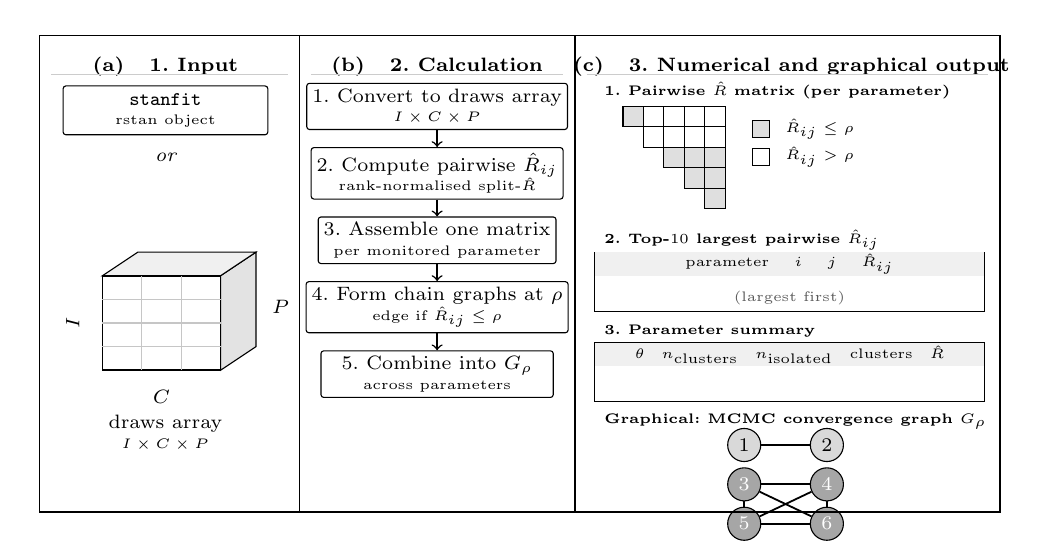
\begin{tikzpicture}[
  x=1cm, y=1cm,
  font=\small,
  chainA/.style={circle, fill=gray!30, draw=black,
                 minimum size=4.2mm, inner sep=0pt, font=\scriptsize},
  chainB/.style={circle, fill=gray!70, draw=black,
                 minimum size=4.2mm, inner sep=0pt, font=\scriptsize,
                 text=white},
  edge/.style={black, line width=0.65pt},
  stagebox/.style={draw=black, rounded corners=1pt,
                   inner sep=2pt, align=center, font=\scriptsize,
                   minimum width=2.95cm, minimum height=0.52cm},
  iobox/.style={draw=black, rounded corners=1pt,
                inner sep=2.5pt, align=center, font=\scriptsize},
  hdr/.style={font=\bfseries\scriptsize, anchor=north},
]

% Fixed canvas so fit()/dividers stay stable
% Panel widths: a [0,3.2], b [3.4,6.7], c [6.9,12.2]
% Vertical: header band y=5.55..5.95; content y=0.15..5.35
\path[use as bounding box] (-0.15,-0.15) rectangle (12.35,6.15);

% =========================================================
% Panel (a): Input   width 3.2
% =========================================================
\begin{scope}

  % Header: letter + title on one line (avoids collision with (a)/(b)/(c))
  \node[hdr] at (1.60, 5.90) {(a)\quad 1.\ Input};

  \node[iobox, minimum width=2.6cm, minimum height=0.62cm]
        at (1.60, 5.10) {%
          \texttt{stanfit}\\[-1pt]
          {\tiny rstan object}%
        };

  \node[font=\scriptsize\itshape] at (1.60, 4.50) {or};

  % Compact draws-array prism; short axis labels only
  \begin{scope}[shift={(0.45,1.55)}]
    % back
    \fill[gray!8]
      (0.35,0.25) -- (1.85,0.25) -- (1.85,1.45) -- (0.35,1.45) -- cycle;
    \draw[gray!55]
      (0.35,0.25) -- (1.85,0.25) -- (1.85,1.45) -- (0.35,1.45) -- cycle;
    % right (P)
    \fill[gray!22]
      (1.85,0.25) -- (2.30,0.55) -- (2.30,1.75) -- (1.85,1.45) -- cycle;
    \draw
      (1.85,0.25) -- (2.30,0.55) -- (2.30,1.75) -- (1.85,1.45) -- cycle;
    % top
    \fill[gray!12]
      (0.35,1.45) -- (1.85,1.45) -- (2.30,1.75) -- (0.80,1.75) -- cycle;
    \draw
      (0.35,1.45) -- (1.85,1.45) -- (2.30,1.75) -- (0.80,1.75) -- cycle;
    % front + I x C grid
    \fill[white]
      (0.35,0.25) -- (1.85,0.25) -- (1.85,1.45) -- (0.35,1.45) -- cycle;
    \draw[line width=0.6pt]
      (0.35,0.25) -- (1.85,0.25) -- (1.85,1.45) -- (0.35,1.45) -- cycle;
    \foreach \x in {0.85,1.35} {
      \draw[gray!45] (\x,0.25) -- (\x,1.45);
    }
    \foreach \y in {0.55,0.85,1.15} {
      \draw[gray!45] (0.35,\y) -- (1.85,\y);
    }
    % short axis ticks/labels (full names in caption)
    \node[font=\scriptsize, rotate=90, anchor=south] at (0.18,0.85) {$I$};
    \node[font=\scriptsize, anchor=north] at (1.10,0.12) {$C$};
    \node[font=\scriptsize, anchor=west] at (2.38,1.05) {$P$};
  \end{scope}

  \node[font=\scriptsize, anchor=north, align=center] at (1.60, 1.35)
        {draws array\\[-1pt]
         {\tiny $I\times C\times P$}};

\end{scope}

% =========================================================
% Panel (b): Calculation   width 3.3
% =========================================================
\begin{scope}[shift={(3.40,0)}]

  \node[hdr] at (1.65, 5.90) {(b)\quad 2.\ Calculation};

  % Stages match the package pipeline:
  % as_draws_array -> pairwise_rhat_calculation -> pairwise_rhat_matrices
  % -> pairwise_rhat_graph -> build_combined_graph
  \node[stagebox] (s1) at (1.65, 5.15)
        {1.\ Convert to draws array\\[-1pt]
         {\tiny $I\times C\times P$}};
  \node[stagebox] (s2) at (1.65, 4.30)
        {2.\ Compute pairwise $\hat{R}_{ij}$\\[-1pt]
         {\tiny rank-normalised split-$\hat{R}$}};
  \node[stagebox] (s3) at (1.65, 3.45)
        {3.\ Assemble one matrix\\[-1pt]
         {\tiny per monitored parameter}};
  \node[stagebox] (s4) at (1.65, 2.60)
        {4.\ Form chain graphs at $\rho$\\[-1pt]
         {\tiny edge if $\hat{R}_{ij}\le\rho$}};
  \node[stagebox] (s5) at (1.65, 1.75)
        {5.\ Combine into $G_{\rho}$\\[-1pt]
         {\tiny across parameters}};

  \draw[->, line width=0.55pt] (s1) -- (s2);
  \draw[->, line width=0.55pt] (s2) -- (s3);
  \draw[->, line width=0.55pt] (s3) -- (s4);
  \draw[->, line width=0.55pt] (s4) -- (s5);

\end{scope}

% =========================================================
% Panel (c): Output   width 5.3
% =========================================================
\begin{scope}[shift={(6.90,0)}]

  \node[hdr, align=center] at (2.65, 5.90)
        {(c)\quad 3.\ Numerical and graphical output};

  % --- 1. Matrix (left) + legend (right), compact ---
  \node[font=\tiny\bfseries, anchor=west] at (0.15, 5.35)
        {1.\ Pairwise $\hat{R}$ matrix (per parameter)};

  \begin{scope}[shift={(0.25,5.15)}]
    \def\cs{0.26}
    \foreach \i/\j in {1/2, 3/4, 3/5, 3/6, 4/5, 4/6, 5/6} {
      \fill[gray!25] ({(\j-1)*\cs}, {-(\i-1)*\cs})
                   rectangle ({\j*\cs}, {-\i*\cs});
    }
    \foreach \i/\j in {1/2,1/3,1/4,1/5,1/6,
                       2/3,2/4,2/5,2/6,
                       3/4,3/5,3/6,
                       4/5,4/6,5/6} {
      \draw ({(\j-1)*\cs}, {-(\i-1)*\cs}) rectangle ({\j*\cs}, {-\i*\cs});
    }
  \end{scope}

  % legend to the right of the matrix (clear of cells)
  \begin{scope}[shift={(2.15,4.55)}]
    \fill[gray!25] (0,0.20) rectangle (0.22,0.42);
    \draw (0,0.20) rectangle (0.22,0.42);
    \node[font=\tiny, anchor=west] at (0.30,0.31) {$\hat{R}_{ij}\le\rho$};
    \draw (0,-0.15) rectangle (0.22,0.07);
    \node[font=\tiny, anchor=west] at (0.30,-0.04) {$\hat{R}_{ij}>\rho$};
  \end{scope}

  % --- 2. Top-10 ---
  \node[font=\tiny\bfseries, anchor=west] at (0.15, 3.45)
        {2.\ Top-$10$ largest pairwise $\hat{R}_{ij}$};
  \draw (0.15,3.30) rectangle (5.10,2.55);
  \fill[gray!12] (0.15,3.30) rectangle (5.10,3.00);
  \node[font=\tiny] at (2.625,3.15)
        {parameter \quad $i$ \quad $j$ \quad $\hat{R}_{ij}$};
  \node[font=\tiny, text=gray!70!black] at (2.625,2.72)
        {(largest first)};

  % --- 3. Summary ---
  \node[font=\tiny\bfseries, anchor=west] at (0.15, 2.30)
        {3.\ Parameter summary};
  \draw (0.15,2.15) rectangle (5.10,1.40);
  \fill[gray!12] (0.15,2.15) rectangle (5.10,1.85);
  \node[font=\tiny] at (2.625,2.00)
        {$\theta$\;\; $n_{\mathrm{clusters}}$\;\; $n_{\mathrm{isolated}}$\;\;
         clusters\;\; $\hat{R}$};

  % --- Graphical: single graph ---
  \node[font=\tiny\bfseries, anchor=west] at (0.15, 1.15)
        {Graphical:\ MCMC convergence graph $G_{\rho}$};

  \begin{scope}[shift={(2.05,0.15)}]
    \node[chainA] (g1) at (0.00, 0.70) {1};
    \node[chainA] (g2) at (1.05, 0.70) {2};
    \node[chainB] (g3) at (0.00, 0.20) {3};
    \node[chainB] (g4) at (1.05, 0.20) {4};
    \node[chainB] (g5) at (0.00,-0.30) {5};
    \node[chainB] (g6) at (1.05,-0.30) {6};
    \draw[edge] (g1) -- (g2);
    \draw[edge] (g3) -- (g4);
    \draw[edge] (g3) -- (g5);
    \draw[edge] (g3) -- (g6);
    \draw[edge] (g4) -- (g5);
    \draw[edge] (g4) -- (g6);
    \draw[edge] (g5) -- (g6);
  \end{scope}

\end{scope}

% =========================================================
% Outer frame + vertical dividers (fixed coordinates)
% =========================================================
\draw[line width=0.6pt] (0.00,0.00) rectangle (12.20,6.05);

% dividers at mid-gaps between panels
\draw[line width=0.5pt] (3.30,0.00) -- (3.30,6.05);
\draw[line width=0.5pt] (6.80,0.00) -- (6.80,6.05);

% light header rule under titles
\draw[gray!40, line width=0.4pt] (0.15,5.55) -- (3.15,5.55);
\draw[gray!40, line width=0.4pt] (3.45,5.55) -- (6.65,5.55);
\draw[gray!40, line width=0.4pt] (6.95,5.55) -- (12.05,5.55);

\end{tikzpicture}%
}% end resizebox
%
\caption{%
\textbf{Workflow of the R package \texttt{pairwiserhat} for computing the
MCMC convergence graph diagnostic.}
The pipeline transforms MCMC draws from any sampler into diagnostic outputs
in three panels: (a)~input, (b)~calculation, and (c)~numerical and graphical
output.
%
(a)~\emph{Input.} Either an \texttt{rstan} \texttt{stanfit} object (top) or
a three-dimensional draws array of iterations~$I$, chains~$C$, and monitored
parameters~$P$ (bottom) is accepted. Both forms are internally standardised
to a common $I\times C\times P$ array, keeping chains distinct throughout so
that the pairwise statistic can be computed between any two chains.
%
(b)~\emph{Calculation.} Five sequential steps, each implemented by a
corresponding R function of the package, realise the pipeline defined in
Section~\ref{sec:theory}: (1) conversion of the input to the common draws
array via \texttt{as\_draws\_array()}; (2) computation of the pairwise
$\hat{R}_{ij}$ between every chain pair and every monitored parameter via
\texttt{pairwise\_rhat\_calculation()}, using the rank-normalised
split-$\hat{R}$ variant of Vehtari~et~al.~\cite{vehtari2021} as the
underlying statistic; (3) assembly of these values into one $C\times C$
symmetric matrix per parameter via \texttt{pairwise\_rhat\_matrices()};
(4) formation of a parameter-level chain graph via
\texttt{pairwise\_rhat\_graph()}, placing an edge between chains~$i$ and
$j$ whenever $\hat{R}_{ij}\le\rho$ for the user-chosen threshold $\rho$;
and (5) combination of the parameter-level graphs across parameters into
$G_{\rho}$ via \texttt{build\_combined\_graph()}, taken here as the
intersection so that an edge is retained in $G_{\rho}$ only if it is
present for every parameter.
%
(c)~\emph{Numerical and graphical output.} Three numerical objects and one
graphical object are returned by \texttt{pairwiserhat()}. The values shown
are those obtained for the Different intercepts variant of Experiment~2.
For reasons of space, the pairwise $\hat{R}$ matrix in~(1) is displayed
for a single parameter, the intercept $b_1$. (1)~A pairwise $\hat{R}$
matrix (top block): shaded cells mark chain pairs~$(i,j)$ with
$\hat{R}_{ij}\le\rho$ and empty cells mark pairs with
$\hat{R}_{ij}>\rho$, so that the block structure of shaded cells exposes
the chain groupings for that parameter at a glance. (2)~A table of the
largest pairwise $\hat{R}_{ij}$ values (middle block), sorted in
descending order, listing the most notable chain-pair disagreements
across all monitored parameters; the five largest rows are shown. (3)~A
parameter-level summary (lower block) reporting, for each monitored
parameter~$\theta$, the number of connected components~$K$, the number of
isolated chains, the chain groups, and the largest within-group pairwise
$\hat{R}_{ij}$. The graphical output is the MCMC convergence graph
$G_{\rho}$ (bottom right), drawn here with eight chains that partition
into two connected components---light-shaded chains~$\{1,2,5\}$ and
dark-shaded chains~$\{3,4,6,7,8\}$---indicating a bimodal posterior in
which two groups of chains have concentrated on different regions of
$b_1$.
}
\label{fig:package-workflow}
\end{figure}
